%%%%%%%%%%%%%%%%%%%%%%%%%%%%%%%%%%%%%%%%%%%%%%%%%%%%%%%%%%%%%%%%%%%%%%%%%%%%%%%%
%2345678901234567890123456789012345678901234567890123456789012345678901234567890
%        1         2         3         4         5         6         7         8

\documentclass[letterpaper, 10 pt, conference]{ieeeconf}  % Comment this line out if you need a4paper

%\documentclass[a4paper, 10pt, conference]{ieeeconf}      % Use this line for a4 paper

\IEEEoverridecommandlockouts                              % This command is only needed if
                                                          % you want to use the \thanks command

\overrideIEEEmargins                                      % Needed to meet printer requirements.

%In case you encounter the following error:
%Error 1010 The PDF file may be corrupt (unable to open PDF file) OR
%Error 1000 An error occurred while parsing a contents stream. Unable to analyze the PDF file.
%This is a known problem with pdfLaTeX conversion filter. The file cannot be opened with acrobat reader
%Please use one of the alternatives below to circumvent this error by uncommenting one or the other
%\pdfobjcompresslevel=0
%\pdfminorversion=4

% See the \addtolength command later in the file to balance the column lengths
% on the last page of the document

% The following packages can be found on http:\\www.ctan.org
%\usepackage{graphics} % for pdf, bitmapped graphics files
%\usepackage{epsfig} % for postscript graphics files
%\usepackage{mathptmx} % assumes new font selection scheme installed
%\usepackage{times} % assumes new font selection scheme installed
\usepackage{amsmath} % assumes amsmath package installed
\usepackage{amssymb}  % assumes amsmath package installed
\usepackage{balance}
\usepackage{xspace}
\usepackage{csquotes}
\usepackage{hyperref}
\usepackage{stmaryrd}
\usepackage{cite}
\usepackage[svgnames,dvipsnames]{xcolor}
\definecolor{shadeGray}{rgb}{0.9,0.95,0.95}
\usepackage[bordercolor=red, backgroundcolor=shadeGray, linecolor=red, textwidth=0.8in, textsize=footnotesize]{todonotes}
\usepackage{listings}
\usepackage{tikz}
\usepackage{pgfplots}
\usepackage{subfig}
\usepackage{paralist}
\lstdefinestyle{corelang}{
  %frame=tb,
  %rulesepcolor=\color{gray},
  rulecolor=\color{gray},
  morekeywords={
  repeat, times, foreach, visit, pick, drop, containing, avoiding, while, strict,
  move, right, move, left, in, every, has, color, shape, possible, if, at, and, or, minus, not
  },%in,
  keywordstyle=[2]\emph,
  keywords=[2]{world, point, robot, item, red, blue, yellow, green, triangle, square, circle},
  sensitive=true,
  morecomment=[l]{//},
  morecomment=[s]{/*}{*/},
  commentstyle=\color{gray},
  showstringspaces=false,
  %columns=fullflexible,
  mathescape=true,
  numberstyle=\tiny,
  basicstyle=\footnotesize\ttfamily,
  numbersep=5pt,
  stepnumber=2,
  numbers=none,                   % where to put the line-numbers
  morestring=[b]"
}
\lstset{style=corelang}
\usepackage[T1]{fontenc}  % this is necessary for beramo to work
\usepackage[scaled=0.80]{beramono}  % our monospace font
\allowdisplaybreaks

\def\pick{\mathtt{pick}}
\def\drop{\mathtt{drop}}
\def\visit{\mathtt{visit}}
\def\avoiding{\mathtt{avoiding}}
\def\while{\mathtt{while}}

\let\proof\relax    % there is an option clash with amsthm with something in IEEEconf
\let\endproof\relax
\usepackage{amsthm}
\usepackage{thmtools}
\declaretheorem[style=definition,qed=$\blacksquare$]{example}

\newcommand{\tool}{Flipper\xspace}

\newcommand{\sem}[2]{\llbracket \texttt{#1}\rrbracket &::= #2}
\newcommand{\bbraces}[1]{\llbracket \texttt{#1}\rrbracket}
\newcommand{\until}[2]{#1\; \mathcal{U}\; #2}

\title{\LARGE \bf Precise but Natural Specifications for Robot Tasks
}


\author{Brendon Boldt$^1$\quad Ivan Gavran$^2$ \quad Eva Darulova$^2$ \quad Rupak Majumdar$^2$%
\thanks{
$^1$Marist College, USA,
$^2$Max Planck Institute for Software Systems, Germany
}%
\thanks{Brendon Boldt was supported by a DAAD RISE Internship.}
}
% \author{Albert Author$^{1}$ and Bernard D. Researcher$^{2}$% <-this % stops a space
% \thanks{*This work was not supported by any organization}% <-this % stops a space
% \thanks{$^{1}$Albert Author is with Faculty of Electrical Engineering, Mathematics and Computer Science,
%         University of Twente, 7500 AE Enschede, The Netherlands
%         {\tt\small albert.author@papercept.net}}%
% \thanks{$^{2}$Bernard D. Researcheris with the Department of Electrical Engineering, Wright State University,
%         Dayton, OH 45435, USA
%         {\tt\small b.d.researcher@ieee.org}}%
% }


\begin{document}



\maketitle
\thispagestyle{empty}
\pagestyle{empty}


%%%%%%%%%%%%%%%%%%%%%%%%%%%%%%%%%%%%%%%%%%%%%%%%%%%%%%%%%%%%%%%%%%%%%%%%%%%%%%%%
\begin{abstract}
We present \tool, a
% community-powered
natural language interface for describing
high level task specifications for robots
that are compiled into robot actions.
\tool starts with a formal core language for task planning that allows
expressing rich temporal specifications and
uses a semantic parser to provide a natural language interface.
\tool provides immediate visual feedback by executing an automatically
constructed plan of the task in a graphical user interface.
This allows the user to resolve potentially ambiguous interpretations.
\tool extends itself via \emph{naturalization}: users of \tool can
define new commands, which are generalized and added as new rules to the core language,
gradually growing a more and more natural task specification language.
%
Unlike other task-specification systems, \tool enables natural language
interactions while maintaining the expressive power and formal precision of a programming language.
We show through an initial user study that natural language interactions and generalization
can considerably ease the description of tasks.
Moreover, over time, users employ more and more concepts outside of the initial core language.
Such extensions are available to the \tool community, and users can use concepts that others have defined.

\end{abstract}


%%%%%%%%%%%%%%%%%%%%%%%%%%%%%%%%%%%%%%%%%%%%%%%%%%%%%%%%%%%%%%%%%%%%%%%%%%%%%%%%

\section{Introduction}

With a long-anticipated migration of robots from factories to homes and offices, bridging
the gap between tasks defined in a high-level, natural language and plans
implemented on physical robots navigating a dynamic environment has become one
of the fundamental challenges in robotics.
% Most robots today are programmed in programming languages and end-user,
% specifically non-programmer, interaction is limited to a few simple settings.
%
Research in planning has focused on precise programming languages for robot tasks.
These languages are expressive, have a clear semantics,
and plans can be automatically generated~\cite{golog, strips, pddl,fainekosTemporalLogicMotionPlanning,hoffmanFF,ankushDrona}.
Unfortunately, the precision of such languages comes with unforgiving syntax.
Thus, it is hard for end-users to translate tasks in a natural language to valid programs.
The usual mechanism to incorporate natural language is to add a fixed set of ``syntactic sugar'' to express
commands in a structured subset \cite{hadasTranslatingStructuredEnglish}.
On the other hand, advances in natural language processing have enabled rich models of natural
language to be built, but the application to robot task planning is usually
limited to a fixed set of the most common scenarios~\cite{hadasProvablyCorrectReactiveControlFromNaturalLanguage,thomasonDialog,kollarDialog}.
Thus, users are either limited to a handful of natual language idioms,
or they can use their language freely, but the robot can only do a handful of actions.

In this paper, we present \tool, a system for end-users to program mobile robots using natural language.
The core of \tool is a high-level formal programming language for task specification.
A \emph{semantic parser} \cite{berantSempre} translates natural language utterances into internal representations for programs,
allowing more flexibility in specifying tasks.
While the core language is always available to programmers,
\tool further allows to extend the capability of the language and parsing through a
process of \emph{naturalization}~\cite{wangVoxelurn}.
Whenever the semantic parser fails to parse an utterance, the user can \emph{define} the
new utterance in terms of a sequence of utterances already understood (i.e., parseable) by the system.
The semantic parser generalizes the definition and adds it as a set of new production rules in the underlying language.
Thus, over time, \tool builds up a large lexicon of defined concepts through user interaction and generalization.
Initial users program in the core language, but build up idioms natural to the domain; future users
can use all concepts defined by the community previously.
Along the way, each parsed form retains the precise semantics of the core language.

Thus, \tool helps bridge the gap between expressive and precise programming languages with restricted syntax
and the flexible but ambiguous natural language.
While defined concepts are the usual way to express a formal language, for example using the library mechanism in a programming
language, \tool exploits two key features of the robotics domain.
First, it can provide quick visual feedback to the user about the \emph{effect} of an utterance by simulating
the plan on the world.
This allows quick resolution of ambiguity.
Second, unlike a library in a general purpose language, in which a programmer parameterizes a function explicitly,
\tool uses grammar induction within the parser to generalize from concrete utterances.
While grammar induction may not be powerful enough for general-purpose computation, it works remarkably well
in the restricted context of planning worlds.


\begin{figure}[t]
\resizebox{\linewidth}{!}{
\includegraphics{flipperSimplestSimulation.png}
}
\caption{Simulation world of \tool}
\label{fig:simulationWorld}
\end{figure}


\smallskip
\noindent
\textbf{Interacting with \tool}
Let us be more specific.
The user of \tool instructs a single robot which moves in a world
consisting of several connected rooms separated by walls, presenting obstacles for the robot.
These rooms contain a number of items with different properties; for simplicity we consider here different
colors and shapes.
The robot can modify this world by moving to free locations,
and by applying a set of actions, such as picking up or dropping items.
Figure~\ref{fig:simulationWorld} shows a simulation of such a world.
The user specifies actions for the robot as an utterance.
For example, the utterance (in the core language) \lstinline{visit world containing item has color blue}
instructs the robot to visit some point that contains a blue item.
\tool parses the utterance into a task specification in the core language, constructs a plan over the simulated
world, and provides visual feedback first, showing what the robot would do.
This is especially useful if there are multiple possible interpretations, e.g., due to ambiguities
in the semantic parsing.
Once the user selects an interpretation, the robot proceeds with an action (ideally,
in the real world; in our current implementation, still in simulation). 

In case the plan is unrealizable, the user receives feedback specifying which primitive part of the
action is not realizable.

It is possible, however, that \tool is not able to parse a command.
For example, the user might state ``visit blue item'' to specify the same task in a more natural way.
In this case, \tool asks the user to define this utterance
in terms of one or more parseable commands already understood by the system.
This is the situation in Figure \ref{fig:simulationWorld}.
\tool generalizes the definition and creates new grammar rules.
Thus, it can now also understand the utterance ``visit red item.''


We have implemented \tool on top of Sempre~\cite{berantSempre}, the trainable semantic parser, its interactive version introduced by the Voxelurn
naturalization tool \cite{wangVoxelurn}, and a temporal path planner.
In a preliminary study on thirteen users (with programming experience), we demonstrate that naturalization
helps specify tasks in a more succinct way, that users define derived concepts as building blocks,
and these derived concepts are reused by later users as their basis for interacting with the system.


% The architecture of \tool has four main components. The first is a formal core language to express temporal objectives in the world (described in the Section \ref{sec:coreLanguage}). The second is an adaptive language component consisting of a semantic parser and a grammar inducer. The role of the semantic parser is to map natural language utterances into their meaning, assign each of them a score according to the model and update the model based on user's choices. Grammar inducer creates new rules from the definitions provided by the user. The adaptive language component is described in the Section \ref{sec:naturalization}.
% The third is a planner that, given a logical representation of a goal, generates a plan for the robot to execute it goal if possible. Finally, a visual user interface provides the user real-time feedback by exhibiting the effect of a plan in a simulated environment.


\section{Core Language and Planning}
\label{sec:coreLanguage}

\tool starts with a \emph{core language} for specifying temporal tasks for a robot in
the abstract world.
\autoref{fig:core-syntax} shows the most interesting subset of the syntax
of the core language.
% the full syntax is available at \url{syntaxurl}.
While the abstract world in which our robot operates may seem relatively simple,
the core language allows expressing many interesting scenarios.
For example, it allows us to express the tasks in~\autoref{fig:core-examples}.

\begin{figure}
  Control flow:
  \begin{lstlisting}
Stmt $\to$ Act $\mid$ Stmt; Stmt $\mid$ repeat Num times Stmt
      $\mid$ foreach point in Area Stmt $\mid$ if Cnd Stmt $\mid$ while Cnd Stmt
  \end{lstlisting}
  Actions:
  \begin{lstlisting}
Act     $\to$ visit Area $\mid$ visit Area while avoiding Area
         $\mid$ move right $\mid$ move left $\mid$ $\ldots$
         $\mid$ ItemAct QItm $\mid$ strict Act
ItemAct $\to$ pick $\mid$ drop
  \end{lstlisting}
  Locations:
  \begin{lstlisting}
Area $\to$ world $\mid$ Pnt $\mid$ [Pnt, Pnt, ..., Pnt] $\mid$ Area containing Itm
     $\mid$ Area and Area $\mid$ Area or Area $\mid$ Area minus Area
Pnt  $\to$ [Num, Num] $\mid$ point
  \end{lstlisting}
  Items:
  \begin{lstlisting}
QItm $\to$ every Itm $\mid$ Itm
Itm  $\to$ item $\mid$ item Fltr
Fltr $\to$ has Prop $\mid$
     $\mid$ Fltr and Fltr $\mid$ Fltr or Fltr $\mid$ not Fltr
Prop $\to$ color C $\mid$ shape S
C    $\to$ red $\mid$ blue $\mid$ green $\mid$ yellow $\mid$ $\ldots$
S    $\to$ triangle $\mid$ square $\mid$ circle $\mid$ $\ldots$
  \end{lstlisting}
  Conditions:
  \begin{lstlisting}
Cnd $\to$ Itm at Area $\mid$ robot has Item $\mid$ robot at Area $\mid$ possible Stmt
  \end{lstlisting}
  \caption{Syntax of core language (subset). Reserved constants and variable
  names are marked in italic.}
  \label{fig:core-syntax}
\end{figure}

\begin{figure}
\begin{example}\label{ex:example1}
Go to a red item and pick it up $\ldots$
\begin{lstlisting}
visit world containing item has color red;
pick item has color red
\end{lstlisting}
$\ldots$ but avoid all circular items along the way
\begin{lstlisting}
visit world containing item has color red
    while avoiding world containing item has shape circle;
pick item has color red
\end{lstlisting}
\vspace{-10pt}
\end{example}

\begin{example}\label{ex:example2}
Gather all red items
\begin{lstlisting}
foreach point in world containing item has color red
    { visit point; pick every item has color red }
\end{lstlisting}
\vspace{-10pt}
\end{example}

\begin{example}\label{ex:example3}
%\item
If possible, form a horizontal line on the floor out of all the items
  the robot currently has (starting at robot's current position and to the right)
    \begin{lstlisting}
strict {while robot has item {drop item; move right}};
    \end{lstlisting}
    \vspace{-10pt}
\end{example}

\begin{example}\label{ex:example4}
Place as many items in a horizontal line as fit.
  \begin{lstlisting}
drop item;
while possible {move right; drop item} {move right; drop item}
  \end{lstlisting}
  \vspace{-10pt}
  \end{example}
\caption{Example commands in the core language}
\label{fig:core-examples}
\end{figure}


Intuitively, the core language interprets a program as a
\emph{temporal goal} for the robot in a grid world.
% \footnote{A full formal definition of our semantics can be found at \url{semanticsurl}.}
The model of the grid world consists of a tuple $(M, I, r)$ where
$M$ is a two-dimensional grid of \emph{points} divided into free points and obstacles,
$I$ is a set of \emph{items}, and $r$ is the robot.
Each item $i \in I$ has associated attributes such as color, shape, and a unique identifier.
Additionally, if it is not held by the robot, it has a position which is a point in $M$.
The robot $r$ has a position in $M$ and holds a possibly empty set of items.

The core language has a set of actions that manipulate the world and combines
actions through standard imperative constructs such as sequencing, conditionals, or loops.
We focus here on the non-standard parts of the language.

%propositions
The propositions of the logical language specify either sets of items or sets of
points, and can be combined using Boolean operations as usual.
The syntactic class ``Locations'' describes sets of points in the grid $M$.
The user can, for instance, start with the entire grid $M$ using
the keyword \lstinline{world} and filter the grid points to those which
contain interesting items using the \lstinline{containing} clause
(see Example~\ref{ex:example1}).
Similarly, the syntactic class ``Items'' describes sets of items.
All items can be selected with the \lstinline{every} keyword and specific items can be chosen
by filtering based on (possibly Boolean combinations) of attributes
(Example~\ref{ex:example2}).

\emph{Actions} modify the state of the world. For example, \lstinline{pick} changes the
world from a state where there is an item $i$ in the current position of the
robot to a world in which the item is being carried by the robot.
Actions can be \emph{temporal}.
The temporal action \lstinline{visit T}, for a set $T\subseteq M$ of points,
requires that the robot is moved to some position in $T$.
The temporal action \lstinline{visit $T$ while avoiding $A$} additionally requires
that along the way the robot never visits any point in $A\subseteq M$
(see Example~\ref{ex:example1}).
They can be written in linear temporal logic (LTL) as $\Diamond T$ and $\until{\lnot A}{T}$,
respectively.
The language is expressive enough to subsume LTL with propositions ranging over points and
items.
% \todo[inline]{IG: how do we encode next (X) operator for visiting a location?}
% RM: move left or move right .. etc


In a complex command, only some part of a command may be realizable.
Consider Example~\ref{ex:example3}: the robot
may be able to move right once but not as many times as it has items.
The default behavior is lenient in that it executes those parts of the command
which are realizable and prints a warning about those which are not.
The \lstinline{strict} modifier allows to specify more rigid behavior that
either performs the \emph{complete} action or no part of it.

In a slight modification of the scenario above, if we want to place as many
items to the right as possible, as in Example~\ref{ex:example4}, then we can use
the \lstinline{while possible S T} construct which executes $T$ repeated while
$S$ is realizable.


% \subsection{Planner and User Feedback}

Given a goal expressed in the core language,
\tool generates an execution plan for the robot to satisfy it in the grid world.
Currently, \tool's planner is based on A* search~\cite{Astar} with Christofides algorithm~\cite{christofides}
for iterated reachability.
However, the planner interface is generic and one can use
a different planner \cite{golog,pddl,hadasLTLMop,ankushDrona,antlab}.
Fast planning is crucial for user interaction and we found
A* to be fast and sufficient to find plans.

The plan generated is shown to the user visually in \tool's graphical interface
by simulating the robot's moves step by step in the UI.
This visual feedback is important to verify that a possibly complex command given to
the robot works as expected.
Furthermore, ambiguities in the grammar can lead to several alternative plans
being generated; the UI enables the user to select the plan which best matches
his or her intentions.





\section{Parsing, Naturalization, and Generalization}
\label{sec:naturalization}

% While the core language is expressive and precise
% its rigid syntax is not suitable for end-users and is at odds
% with the flexibility of natural language.
% Therefore, \tool enables its users to
% extend the grammar of the core language, or
% \emph{naturalize}~\cite{wangVoxelurn} it.
% Users can define the meaning of new utterances, and \tool generalizes their definitions into new grammar production rules.

We now describe how naturalization works in \tool.
We start by showing two examples of naturalization and then
explain the inner mechanism of the naturalization process.

\begin{example}\label{ex:pick-3-items}
Suppose a user writes the command \lstinline{pick 3 items}. Since this is not a valid program
in the core language, \tool asks for a definition.
Suppose the user responds with \lstinline{repeat 3 times pick item}.
From this, \tool's grammar induction module now induces the following
two grammar rules:
\begin{lstlisting}
Act $\to$ pick Num items      ::= repeat Num times pick item
Act $\to$ ItemAct Num items ::= repeat Num times ItemAct item
\end{lstlisting}
%
Note that these rules are a generalization of the user-provided definition.
Thus, when the next user issues the command \lstinline{drop 2 items}, the semantic parser
will be able to parse it and \tool will successfully execute it.
\end{example}

\begin{example}
\label{ex:definingAFunction}
Naturalization not only helps accommodate many different language styles, it can also significantly simplify programs.
Consider the task of distributing items of different colors to different rooms.
Conceptually, this is fairly simple: the robot should first gather all red items and put them into \lstinline{room1},
then do the same for the blue items and \lstinline{room2} and so on.
Figure \ref{fig:coreLanguageDefinitionOfSortingOnColors} shows an implementation of this specification in the core language.
Each marked part corresponds to gathering items of a specific color (as in Example~\ref{ex:example2}) and bringing
them to a specific room.
Clearly, there is a significant amount of redundancy.
\begin{figure}[t!]
  \begin{lstlisting}[frame=leftline,xleftmargin=15pt, xrightmargin=15pt]
foreach point in world containing item has color red
  {visit point; pick every item has color red };
visit room1; drop every item has color red;
  \end{lstlisting}

  \begin{lstlisting}[frame=leftline,xleftmargin=15pt, xrightmargin=15pt]
foreach point in world containing item has color green
  {visit point; pick every item has color green};
visit room2; drop every item has color green;
  \end{lstlisting}

  \begin{lstlisting}[frame=leftline,xleftmargin=15pt, xrightmargin=15pt]
foreach point in world containing item has color blue
  {visit point; pick every item has color blue};
visit room3; drop every item has color blue;
  \end{lstlisting}

  \begin{lstlisting}[frame=leftline,xleftmargin=15pt, xrightmargin=15pt]
foreach point in world containing item has color yellow
  {visit point; pick every item has color yellow};
visit room4; drop every item has color yellow
  \end{lstlisting}
\caption{Sorting items based on colors using the core language}
\label{fig:coreLanguageDefinitionOfSortingOnColors}
\end{figure}

With naturalization, we can accomplish the same task by first defining
\lstinline{gather red} as
  \begin{lstlisting}
foreach point in world containing item has color red
  {visit point; pick every item has color red}
  \end{lstlisting}
Then using this new command, we define \lstinline{red to room1} as
\begin{lstlisting}
gather red; visit room1; drop every item has color red
  \end{lstlisting}
and finally we can accomplish our complete task with
\begin{lstlisting}
red to room1; green to room2; blue to room3; yellow to room4
\end{lstlisting}
%
If we next want to put all items of different shapes to different rooms,
the generalization allows us to re-use the commands defined above and simply
write:
  \begin{lstlisting}
triangle to room1; circle to room2; square to room3
  \end{lstlisting}
\end{example}

Thus, the naturalization process is a convenient way of
giving alternative names to existing concepts and defining functions by example,
akin to extending a programming language through new functions, but with two differences.
Unlike usual programming languages, which require every definition to be in the core syntax,
we use a \emph{semantic parser} to allow for relaxed syntax and natural linguistic styles.
Second, the user always provides concrete values and the underlying system takes care of parameter inference
through \emph{grammar induction}.
These features make the overall system more accessible to non-programmers over time.
% but it still requires them to consult the manual of the core-language from time to time.
%
% This is, however, only one part of the story.
% More exciting is the fact that newly defined concepts can be shared across a community of users.
% The idea is that people will likely have similar linguistic expressions for similar commands.
% Hence, users who join a community later will only rarely need to define their own concepts.
% Indeed, assuming that a robot works in a particular context, i.e. the same users
% use it for an unbounded number of different but similar tasks, \tool gradually
% becomes a pure natural language interface.
%
Moreover, each defined notion is available for use in the future and to different users.
Thus, over time, \tool develops the common linguistic style and phraseology of its user base.

We now describe the semantic parser and grammar induction.
%
% Our semantic parser and grammar induction modules reuse the corresponding
% modules from Voxelurn~\cite{wangVoxelurn} and its
% dependencies~\cite{zettlemoyerSentencesToLogicalForm,berantSempre}. We now
% provide necessary background on these methods and explain the adaptations that we
% introduced.


\subsection{Semantic Parsing}
Semantic parsing
is the task of turning a natural language utterance ($x$) into a
ranked list of formal representations (such as a logical formula, a formal specification, or a
formal language expression) for actions~\cite{liangSemanticParsers}.
For example, if $x = \text{``How much is three times four?''}$,
a possible intermediate representation is $3*4$ and a
resulting action is computing the product.
In \tool, the role of the semantic parser is to turn an utterance $x$
into a ranked list of temporal goals represented in the core language.
The corresponding actions are the plans for these goals.
\tool uses the interactive semantic parser presented in~\cite{wangVoxelurn}.
The semantic parser outputs a ranked list because utterance parses may be ambiguous.
In \tool, ambiguous derivations can occur
due to ambiguities in the core language
or due to conflicting definitions (e.g., by different users) for the same utterance.
An example for the former is \lstinline{pick item not has color red and has shape circle}
which could mean either
\lstinline |pick item not {has color red and has shape circle} | or \lstinline |pick item {not has color red} and {has shape circle}|.
The latter occurs when for one user
\lstinline{take red} means \textit{pick up a red item from the
current field}, but for the other \textit{find a red item and then pick it up}.

To rank the potential parses, the parser uses a model $p_\theta(d | x, u)$
which gives the probabilities over derivations $d$ given the utterance $x$ by the user $u$,
using a set of parameters $\theta$.
\tool then offers three best-ranked derived programs to the user who
visually inspects their execution in simulation.
Based on the user's choice, the model's parameters $\theta$ are updated.
The set of features influencing the
model include whether the rule comes from the core language or it is induced,
whether the author of the rule is the same person as $u$, the user providing the
utterance, etc.

%\begin{figure}
%\tikzstyle{vertex}=[draw,rectangle,minimum size=10pt,inner sep=2pt]
%\tikzstyle{every node}=[font=\small]
%\begin{tikzpicture}[font=\sffamily,thick, level/.style={sibling distance=47mm/#1}]
%    \node[vertex] {Act: foreach point in Area Act }
%        child {
%            node[vertex] {Area: world?Prop}
%            child {
%                node[vertex] {Prop: Shape}
%                child{
%					node[vertex]{Shape: circle}
%                }
%            }
%        }
%        child {
%                node[vertex] {Act: Act; Act}
%                child { node[vertex] {Act: visit point} }
%                child {
%                    node[vertex] {Act: pick QItm}
%                    child {
%                    		node[vertex] {QItm: every item?Prop}
%                    		child{
%                 			node[vertex] {Prop: Shape}
%				                child{
%									node[vertex]{Shape: circle}
%				                }
%                    		}
%                    	}
%                }
%            }
%      ;
%\end{tikzpicture}
%\caption{Parse tree for the utterance \lstinline{gather circle}}
%\label{fig:parseTree}
%\end{figure}

%The underlying semantic parser Sempre~\cite{berantSempre} allows to choose
%between two natural language analyzers that perform a preprocessing step: a
%simple natural language analyzer and a more involved one that uses Stanford
%CoreNLP tools~\cite{manningCoreNLP}. In the current implementation we use the
%simpler one.
%\todo[inline]{ED: the above paragraph seems a bit out of place}


\subsection{Grammar Induction}
\label{subsec:grammarInduction}

When the semantic parser is unable to parse an utterance,
it asks the user to provide a definition.
The grammar induction module generalizes the definition for a particular
utterance into a new grammar rule.
The grammar induction module receives an utterance $x$, and its definition $y$.
For instance, in Example~\ref{ex:pick-3-items}, \lstinline{$x=$ pick 3 items} and
\lstinline{$y =$ repeat 3 times pick item}.
While $y$ must be fully parseable using the current grammar rules, only some parts of $x$ may be parseable.
In order to induce new rules, we are interested in finding \textit{matches}---parseable spans appearing in both $x$ and $y$.
A set of non-overlapping parsable spans is called a \emph{packing}.

New grammar rules are generated in one of the following three ways:
\begin{itemize}
 \item[\bf simple packing:] only primitive values are matched (in \tool those
 are directions, numbers, colors, shapes and points). Once matched, a new rule
 is introduced in the form of $C_y \rightarrow x[a_1/A_1,\ldots, a_k/A_k]$,
 where $C_y$ is the category of $y$ and $x[a_1/A_1,\ldots, a_k/A_k]$ is the
 utterance with all occurrences of primitive value $a_i$ replaced by its
 category $A_i$. For Example~\ref{ex:pick-3-items} the only primitive match would be number 3. Therefore, a new rule will be added to the grammar \lstinline{Act -> pick Num items} with the same action specification as \lstinline{repeat Num times pick item}

 \item[\bf best packing:] considers maximal packings, i.e. those that would
 become overlapping by adding any other derivation. This method chooses the
 packing that scores the best under the model $p_\theta$. Subsequently, a rule
 induction (similar to the one described for simple packing) based on the
 matching between $y$ and the found best maximal packing is performed.
 As an example, take $x = \text{\lstinline{pick item has color green and shape circle}}$ and
$y = \text{\lstinline{pick item has color green and has shape circle}}$. Two maximal packings of $x$ are $\alpha$ and $\beta$

 \[
 \ooalign{
 $\overbrace{\text{pick item has color green}}^{A_\alpha}\text{and}\overbrace{\text{shape}}^{B_\alpha}\overbrace{\text{circle}}^{C_\alpha}$\cr
 $\underbrace{\phantom{\text{pick}}}_{A_\beta}\underbrace{\phantom{\text{item has color green}}}_{B_\beta} \phantom{\text{and}} \underbrace{\phantom{\text{shape}}}_{C_\beta}\underbrace{\phantom{\text{circle}}}_{D_\beta}$\cr
 }
 \]
%
 and their matching parts in $y$

 \[
 \ooalign{
 $\overbrace{\text{pick item has color green}}^{A_\alpha}\text{and \textcolor{red}{has}}\overbrace{\text{shape}}^{B_\alpha}\overbrace{\text{circle}}^{C_\alpha}$\cr
 $\underbrace{\phantom{\text{pick}}}_{A_\beta}\underbrace{\phantom{\text{item has color green}}}_{B_\beta} \phantom{\text{and \textcolor{red}{has}}} \underbrace{\phantom{\text{shape}}}_{C_\beta}\underbrace{\phantom{\text{circle}}}_{D_\beta}$\cr
 }
 \]
%
The best of all maximal packings (there are more than just $\alpha$ and $\beta$) is $\beta$, so a new rule is produced
\lstinline{Act $\to$ ItemAct item Fltr and Prop}

 \item[\bf alignment:] Utterance $x$ and derivation $y$ are compared and if they align almost perfectly, a new rule is produced.
As an example, for \lstinline{$x =$ throw item} and \lstinline{$y =$ drop item}, a new rule is added
 \lstinline{ItemAct $\to$ throw $::=$ drop}.
\end{itemize}
%
In order to avoid unintended generalizations, the implementation
of grammar induction introduces many restrictions for the above three methods, 
such as stopping the search after finding the
first alignment match, and limiting the differences in size between matches.
We dropped some of those restrictions in order to induce more rules,
and observed no significant penalty on overall user experience.
Unintended generalization happens nonetheless, but their effect is dampened when
users choose between multiple offered behaviors, which dynamically updates the
parameters of the model in the semantic parser.
This effectively removes unintended generalizations from the system over time.

We add one additional new improvement to the process of grammar induction.
Sometimes users, especially those not very adept at programming in the core
language, will define their utterances specific to the state of the world rather
than in the most general form.
In Example~\ref{ex:pick-3-items}, such a specific definition might be
\lstinline{pick 3 items $=$ pick item; pick item; pick item}. This definition,
however, will not generalize to
\lstinline{pick 2 items} using any of the described methods.
A solution would be to explore the space of semantically equivalent definitions and feed them as an additional
input into the previous three methods to obtain more meaningful new rules.
Currently, the exploration is limited only to rule-based search for hidden loops. In our
example, the definition equivalent to \lstinline{pick item; pick item; pick item}
would be \lstinline{repeat 3 times pick item}, which would generalize
correctly. The mentioned changes turned out to be useful in practice.

\section{Evaluation}

\tool is available at \url{flipper.mpi-sws.org}. It consists of a backend
responsible for semantic parsing, a frontend that visually demonstrates to the user the effect of each interpretation of an utterance (both based on \cite{wangVoxelurn}), and a planning module.
%\footnote{The code is available at \url{github/gitlab for both repositories}}.
As our core language is a mixture of concepts typical for
imperative programming (e.g.\ \lstinline{move left}) and an \textit{avoid-until-
reach} temporal specification, we use an adapted version of the
$A^*$~\cite{hipsterHeuristicPlanner} algorithm as our planner. 
% Depending on a deployment scenario and language requirements, we could choose a different
% planner supporting declarative specifications~\cite{metricFF,hadasLTLMop,antlab}.

\subsection{Goal of Evaluation}
Our final goal is to create a system which people with different levels of
proficiency in the core language would use. Envisioned users range from
\emph{expert users}, i.e., those that define new commands to make the
communication with the robot simpler, all the way to those who do not know the
language at all. The latter take advantage of commands that \emph{sound as if they
should work}, and which were defined by other users of the system.

In the evaluation we were thus interested in two properties:
\begin{enumerate}
	\item whether or not users are inclined to define new commands and whether
		those commands make their work easier, and
	\item how much they are able to benefit from other people's definitions
		(without knowing them in advance).
\end{enumerate}
The first property corresponds to the ability to define functions in a programming language,
except that \tool generalizes definitions from examples. The second property
describes how much closer the system gets to pure natural-language interface if
there is a number of active expert users. We thus want to test our intuition
that different people use similar linguistic expressions for similar commands
and that is why they do not have to be aware of existing definitions.

\subsection{Setup}
We created a list of 21 tasks. The tasks levels ranged from easy (e.g.
``get one green square'') to difficult (e.g. ''bring all red items to a
room that contains a yellow square''). The list of all tasks, as well as
all our experimental data is available at \tool's website.
% \todo[inline]{@Ivan: reminder to put list of tasks on website}
%
We recruited thirteen participants, all with prior programming experience but without any
knowledge of the system, and split them into three groups:
\begin{itemize}
	\item Group $A$ (4 members) was only allowed to use the core language,

	\item Group $B$ (6 members) could additionally define their own concepts,

	\item Group $C$ (3 members) additionally had access to concepts defined by two
		expert users (familiar with the system and the language) as well as by other
		participants from group C in real time.
\end{itemize}
%
At the start of the experiment, each group had 30 minutes to familiarize themselves with the core language by following a tutorial. 
%\footnote{tutorial is available at \url{TUTORIALURL}}.
Then participants were instructed to solve the 21 tasks as they saw fit, i.e., not necessarily in the most general way.
The average time needed to solve all tasks was 90 minutes (no deadline was set). 
For each participant, we measured the number of accepted commands, i.e., the syntactically 
correct ones coming either from the core or the induced language,
and the total number of words, defined concepts, and induced commands used to finish all tasks. 
For induced commands we additionally distinguish whether they were defined by the same or by another participant.

%\paragraph*{\textbf{Difficulty of Learning the Core Language}}

Learning any new programming language in half an hour is a nontrivial task. In
our experiment, the average number of successfully parsed queries in group $A$
(only using the core language) was 75\%, with some differences between
the participants (63\%, 70\%, 77\% and 90\%).


\subsection{Results}

\paragraph*{\textbf{Usefulness of Naturalization}}
To assess the usefulness of naturalization, we compare the total number of
tokens needed to finish the tasks for the different groups
(\autoref{fig:numTokens}), and how often participants in groups $B$ and $C$ used
defined concepts (\autoref{fig:groupBAndCCoreVsInduced}).
The latter shows that participants who were allowed to define their own concepts
also used that opportunity.
When comparing the participants from groups $B$ and $C$ to those of group $A$, 
it is clear that the participants who were able to use naturalization end up with less work in 
terms of total number of tokens needed to finish the tasks. 
Specifically, the average number of tokens needed for groups $B$ and $C$ is 1156, 
while for group $A$ it is 1765. 
This takes into account all tokens, also the ones from unsuccessful commands. 
We include these, as some number of unsuccessful commands by groups that use naturalization comes from trying 
out commands they believed might be defined by others.
Only considering successful commands, groups $B$ and $C$ use in total 738 tokens compared to 1287 in group $A$, 
i.e., an improvement of 43\% with respect to the usage of the core language only.
These results suggest that naturalization reduces users' effort. 
It is important to note that individual performances of participants within a single group vary, as shown in~\autoref{fig:numTokens}.

\paragraph*{\textbf{Naturalization across Users}}
Participants in group $C$ had access to the concepts defined by others. Interestingly, these
participants adopted different strategies. While they were on average more likely to use induced
language than the core language (43 vs.\ 35 commands), only one participant relied primarily on the induced language.
The other two users used slightly more core than induced language (see~\autoref{fig:groupBAndCCoreVsInduced}).
The main point of the experiment for group $C$ was to see whether the existence of previously defined concepts is helpful.
We first notice that participants were indeed using concepts defined by others (\autoref{fig:groupCRulesInducedBySelfVsOthers}). 
Again, the numbers differ among participants. 
By looking closer at the kinds of commands issued by each participant, we see that these differences 
stem from their individual styles: participant $C2$ chose to try small building blocks that matched the style of 
the two expert users whose definitions were available to group $C$. 
Participant $C3$, on the other hand, used commands similar to the core language.
%\footnote{All commands by all experiment participants are available at \url{URLFORALLDATA}}.
Curiously, after the experiment two participants (C1 and C3) claimed that they have not much used the predefined rules 
and that they ended up using almost exclusively self-defined concepts (in addition to the the core language). 
The data, however, told a different story (\autoref{fig:groupCRulesInducedBySelfVsOthers}): $C1$ roughly equally used rules defined by others and by himself, while $C3$ 
used much more induced rules. 
Upon inspection of the logs, it turned out that on many occasions they believed they were using the core language, while in fact they used induced concepts
defined by others
(e.g. \lstinline{move 2 right} or \lstinline{drop all blue items}).

\paragraph*{\textbf{Types of Defined Concepts}}
Upon closer inspection of the concepts the participants defined, we see that a majority falls into two categories:
\begin{inparaenum}[(1)]
\item simplifying individual commands and
\item defining functions.
\end{inparaenum}
%
Examples for the first case are
\lstinline{pick green square} defined as \lstinline{pick item has color green} and
\lstinline{visit empty space} defined as \lstinline$visit world minus {world containing item}$.

For the second case a simple example is
\lstinline{visit both triangle and green} defined as
\begin{lstlisting}
visit { {world containing item has shape triangle} and
  {world containing item has color green} }
\end{lstlisting}
There were also function definitions that involved previous function definitions,
such as \lstinline{line red} being defined as
\lstinline$fetch all red; while {robot has item} {drop item; move left}$.
Another noticeable phenomenon was that group C had to define some concepts already defined by others.
The reason was small variations in the utterances (e.g. \lstinline{pick red} vs.\
\lstinline{take a red} vs.\ \lstinline{take a red item}) which can be caught by a more
comprehensive natural language processing module.


\begin{figure}[t!]

		\resizebox{\linewidth}{!}{
		\centering
				\begin{tikzpicture}
				\begin{axis}[
				ticklabel style = {font=\tiny},
				    ybar,
				    bar width = 3,
				    area legend,
				    %enlargelimits=0.15,
				    legend style={at={(0.5,-0.15)},
				      anchor=north,legend columns=-1},
				    ylabel={\# tokens},
				    symbolic x coords={A1, A2, A3, A4, B1,B2,B3,B4,B5,B6,C1,C2,C3},
				    xtick=data,
	%			    nodes near coords,
				    ]
				\addplot coordinates {(A1,1105 ) (A2,1035 ) (A3,1853) (A4, 1156) (B1, 375) (B2, 957) (B3, 549) (B4, 1063) (B5, 970) (B6, 985) (C1,649) (C2,622) (C3,478)};
				\addplot coordinates {(A1,1398 ) (A2,1220 ) (A3,2790) (A4, 1654) (B1, 760) (B2,1364) (B3, 822) (B4, 1471) (B5, 1578) (B6, 1270) (C1,1098) (C2,982) (C3,1061)};
			%	\addplot coordinates {(B1,30) (B2, 61) (B3, 29) (B4, 107) (B5, 80) (B6, 158) (C1,46) (C2,13) (C3,48)};
				\legend{successful commands, all commands}
				\end{axis}
				\end{tikzpicture}
	}
	\caption{Total number of tokens used per participant}
	\label{fig:numTokens}
	\end{figure}






\begin{figure}[t!]
		\resizebox{\linewidth}{!}{
		\centering



				\begin{tikzpicture}
				\begin{axis}[
				    ybar,
				    bar width = 5,
				    area legend,
				    %enlargelimits=0.15,
				    legend style={at={(0.5,-0.15)},
				      anchor=north,legend columns=-1},
				    ylabel={\# commands},
				    symbolic x coords={B1,B2,B3,B4,B5,B6,C1,C2,C3},
				    xtick=data,
	%			    nodes near coords,
				    ]
				\addplot coordinates {(B1, 38) (B2, 64) (B3, 47) (B4, 6) (B5, 45) (B6, 62) (C1,37) (C2,65) (C3,28)};
				\addplot coordinates {(B1,30) (B2, 61) (B3, 29) (B4, 107) (B5, 80) (B6, 158) (C1,46) (C2,13) (C3,48)};
				\legend{induced, core}
				\end{axis}
				\end{tikzpicture}


	}

	\caption{Core-language commands vs induced commands for groups B and C}
	\label{fig:groupBAndCCoreVsInduced}
	\end{figure}


\begin{figure}[t!]
	\resizebox{\linewidth}{!}{
		\centering
		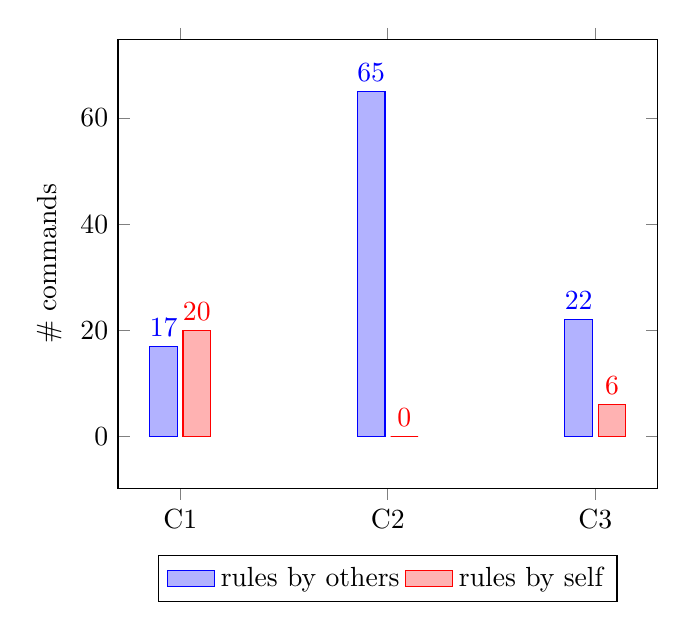
\begin{tikzpicture}
			\begin{axis}[
			    ybar,
			    area legend,
			    enlargelimits=0.15,
			    legend style={at={(0.5,-0.15)},
			      anchor=north,legend columns=-1},
			    ylabel={\# commands},
			    symbolic x coords={C1,C2,C3},
			    xtick=data,
			    nodes near coords,
			    ]
				\addplot coordinates {(C1,17) (C2,65) (C3,22)};
				\addplot coordinates {(C1,20) (C2,0) (C3,6)};
				\legend{rules by others, rules by self}
			\end{axis}
		\end{tikzpicture}
	}
	\caption{Using rules induced by others vs. self-induced rules}
	\label{fig:groupCRulesInducedBySelfVsOthers}
\end{figure}


%\begin{figure}[t!]
%		%\resizebox{\linewidth}{!}{
%		\centering
%		\subfloat[][Core language commands vs induced commands]{\resizebox{0.5\linewidth}{!}{
%
%				\label{fig:groupCCoreVSInduced}
%				\begin{tikzpicture}
%				\begin{axis}[
%				    ybar,
%				    area legend,
%				    enlargelimits=0.15,
%				    legend style={at={(0.5,-0.15)},
%				      anchor=north,legend columns=-1},
%				    ylabel={\# commands},
%				    symbolic x coords={C1,C2,C3},
%				    xtick=data,
%				    nodes near coords,
%				    ]
%				\addplot coordinates {(C1,37) (C2,65) (C3,28)};
%				\addplot coordinates {(C1,46) (C2,13) (C3,48)};
%				\legend{induced, core}
%				\end{axis}
%				\end{tikzpicture}
%
%	}
%			}
%\subfloat[][Using rules induced by others vs. self-induced rules]{\resizebox{0.5\linewidth}{!}{
%
%				\label{fig:groupCRulesInducedBySelfVsOthers}
%				\begin{tikzpicture}
%				\begin{axis}[
%				    ybar,
%				    area legend,
%				    enlargelimits=0.15,
%				    legend style={at={(0.5,-0.15)},
%				      anchor=north,legend columns=-1},
%				    ylabel={\# commands},
%				    symbolic x coords={C1,C2,C3},
%				    xtick=data,
%				    nodes near coords,
%				    ]
%				\addplot coordinates {(C1,17) (C2,65) (C3,22)};
%				\addplot coordinates {(C1,20) (C2,0) (C3,6)};
%				\legend{rules by others, rules by self}
%				\end{axis}
%				\end{tikzpicture}
%
%	}
%			}
%	\caption{Usage of induced rules in group C}
%
%\end{figure}

\section{Related work}

There are many systems commanding or communicating naturally with robots as well as creating programming
languages for robots usable by non-programmers, starting with the seminal work in SHRDLU~\cite{shrdlu},
and continuing over the years~\cite{kollarDialog,thomasonDialog,roboFlow}.
% We believe that natural language---if done right---is the most promising interface with robots (or machines in general).
% \todo[inline]{ED: maybe too strong? perhaps just say, it's an alternative?}
% Kollar et al.~\cite{kollarDialog} and Thomason et al.~\cite{thomasonDialog} recognize the
% need for a dialog between a robot and a human in order for the robot to
% understand the human's intentions and to build trust in mutual understanding.
For example, Thomason et al.~\cite{thomasonDialog} demonstrate a system in which
utterances are mapped to $\lambda$-calculus computations and the robot 
fills in the gaps in a simple \textit{action-patient-recipient} pattern, supporting
navigation and delivery.
%
%  whereas \tool's robot actions can be of arbitrary complexity.
%\todo[inline]{ED: how is SHRDLU related to the other works? I would skip the
%sentence about the need for trust. Sounds subjective to me.}
%\todo[inline]{ED: what is an action-patient-recipient pattern? Is there a different
%word for patient?}
%\todo[inline]{IG: it is a type of thematic relation, a concept from linguistics. At least two papers from our related work are using this term}
%Alexandrova et al.\cite{roboFlow} created a flow-based visual programming language, balancing
%intuitiveness and expressivity. 

Formal and logical languages for planning have a long research tradition in AI and formal methods.
Recently, the work by Kress-Gazit et
al.~\cite{hadasTranslatingStructuredEnglish,hadasLTLMop,
hadasProvablyCorrectReactiveControlFromNaturalLanguage} focuses on translating
natural language into linear temporal logic to bridge the gap from users to formal methods
tools.
One project uses a pipeline of general-purpose NLP 
methods~\cite{hadasProvablyCorrectReactiveControlFromNaturalLanguage}, with VerbNet~\cite{schulerVerbnet}
at the core of semantic interpretation. A robot is additionally able
to give an answer to what it is currently doing, based on the natural language
to LTL translation tree, as well as to explain why an action is unrealizable. A
limitation is, however, that the set of actions a robot can perform is still
restricted to implemented semantic behaviours. On the other hand,~\cite{hadasTranslatingStructuredEnglish}
can process any (GR(1)) LTL specification, but the burden is on the human to use
only \emph{structured English}. \tool accomplishes both, with the tradeoff 
that at least some of the users are able to learn the core language.

Tellex et al.~\cite{tellexGrounding} solve the problem of grounding utterances
from the command to objects in space by introducing a hierarchical structure
that connects expressions such as \emph{beside the truck} and \emph{beside the
box}. Paul et al.~\cite{paulGrounding} solve the same problem, but support
abstract expressions such as \emph{first cube in the second row}. This line of
work is connected to the one described in the previous paragraph in the work by
Boteanu et al.~\cite{boteanuVerifiableGrounding}---there the grounding
problem is put in the context of reactive temporal commands. In this line of
work, unlike in \tool, the robot cannot be taught new concepts. On the other hand,
\tool does not support talking about abstract spatial relations between items
in its world. To support this, \tool's core language would need to be modified
(and one could then use the mentioned techniques).

\tool is inspired by and based upon the work on naturalization of formal
languages by Wang et al.~\cite{wangVoxelurn}, which considers
a block world where a user can build various shapes of different
colors. The application of naturalization to a robot world introduces new
challenges: the language contains declarative and unrealizable
commands and dynamic behavior that changes the state of the world.
A similar approach of learning the language from users is presented in~\cite{azariaLia}, but in the context of personal
assistants. 
Iyer et al.~\cite{iyerLearningNeuralSemanticParser} use user's feedback to 
minimize the effort needed for additional annotation of data and iteratively improve their semantic parser 
that translates natural language utterances to SQL queries. 
Beltagy and Quirk~\cite{beltagyIFTT} train a model (an ensemble of a neural network and logistic
regression) that translates a task description from an IFTTT dataset into
executable representations. They show several ways to improve the performance, the
most interesting of which is creating synthetic data by paraphrasing task
descriptions. Work by Lin et al.~\cite{linTelina} has a similar motivation:
starting with questions from popular programming-help websites that describe
programmers' intentions, they devise bash one-liners accomplishing it. 
This kind of work enables semantic parsing from 
less direct instructions, but is not easily adaptable to users interactively giving clues to the 
system about the meaning of the utterance.
None of these papers targeted the robotics domain.


\section{Conclusion}

% Effectively communicating with robots has been a long-standing research problem.
We have shown that naturalizing a domain-specific programming language is well suited
to provide a natural language interface to robot task specifications.
\tool provides the precision, expressivity, and extensibility of a programming
language, while ensuring a natural experience for humans.
\tool adapts its language to its users by learning new concepts from them. 
The results of our initial evaluation are encouraging and suggest
that a formal language for instructing robots can be turned with community
effort into a \emph{domain specific natural language}.

To accomplish our goal to its full extent, a few challenges remain to be solved.
The first one is lowering the entry bar to the system in its early phase, i.e.
learning the core language.
This could be accomplished by adding syntactic sugar or a specialized interface,
while keeping the rich formalism as a latent representation of
the space of robot tasks.
% A second direction is to include more sophisticated NLP techniques on top of the
% naturalization process such as lemmatization, rephrasing of definition heads, and
% rephrasing of the initial formal language.
Finally, the user experience of \tool can be improved to offer explanations for
unparseable utterances, better depict alternate interpretations of an utterance
which have the same execution, or auto-complete for available pre-defined concepts.


\balance
% \addtolength{\textheight}{-12cm}   % This command serves to balance the column lengths
                                  % on the last page of the document manually. It shortens
                                  % the textheight of the last page by a suitable amount.
                                  % This command does not take effect until the next page
                                  % so it should come on the page before the last. Make
                                  % sure that you do not shorten the textheight too much.

%%%%%%%%%%%%%%%%%%%%%%%%%%%%%%%%%%%%%%%%%%%%%%%%%%%%%%%%%%%%%%%%%%%%%%%%%%%%%%%%



%%%%%%%%%%%%%%%%%%%%%%%%%%%%%%%%%%%%%%%%%%%%%%%%%%%%%%%%%%%%%%%%%%%%%%%%%%%%%%%%



%%%%%%%%%%%%%%%%%%%%%%%%%%%%%%%%%%%%%%%%%%%%%%%%%%%%%%%%%%%%%%%%%%%%%%%%%%%%%%%%



%%%%%%%%%%%%%%%%%%%%%%%%%%%%%%%%%%%%%%%%%%%%%%%%%%%%%%%%%%%%%%%%%%%%%%%%%%%%%%%%



\begin{thebibliography}{10}

\bibitem{golog}
H.~Levesque, R.~Reiter, Y.~Lesp{\'{e}}rance, F.~Lin, and R.~Scherl, ``{GOLOG:}
  {A} logic programming language for dynamic domains,'' {\em J. Log. Program.},
  vol.~31, no.~1-3, 1997.

\bibitem{strips}
R.~Fikes and N.~J. Nilsson, ``{STRIPS:} {A} new approach to the application of
  theorem proving to problem solving,'' {\em Artif. Intell.}, vol.~2, no.~3/4,
  1971.

\bibitem{pddl}
M.~Ghallab, C.~Aeronautiques, C.~K. Isi, and D.~Wilkins, ``{PDDL}: The planning
  domain definition language,'' Tech. Rep. CVC TR98003/DCS TR1165, Yale Center
  for Computational Vision and Control, 1998.

\bibitem{fainekosTemporalLogicMotionPlanning}
G.~E. Fainekos, A.~Girard, H.~Kress{-}Gazit, and G.~J. Pappas, ``{Temporal
  Logic Motion Planning for Dynamic Robots},'' {\em Automatica}, vol.~45,
  no.~2, pp.~343--352, 2009.

\bibitem{hoffmanFF}
J.~Hoffmann and B.~Nebel, ``{The FF Planning System: Fast Plan Generation
  Through Heuristic Search},'' {\em CoRR}, vol.~abs/1106.0675, 2011.

\bibitem{ankushDrona}
A.~Desai, I.~Saha, J.~Yang, S.~Qadeer, and S.~A. Seshia, ``{DRONA: a Framework
  for Safe Distributed Mobile Robotics},'' in {\em ICCPS}, 2017.

\bibitem{hadasTranslatingStructuredEnglish}
H.~Kress{-}Gazit, G.~E. Fainekos, and G.~J. Pappas, ``{Translating Structured
  English to Robot Controllers},'' {\em Advanced Robotics}, vol.~22, no.~12,
  pp.~1343--1359, 2008.

\bibitem{hadasProvablyCorrectReactiveControlFromNaturalLanguage}
C.~Lignos, V.~Raman, C.~Finucane, M.~P. Marcus, and H.~Kress{-}Gazit,
  ``{Provably Correct Reactive Control from Natural Language},'' {\em Auton.
  Robots}, vol.~38, no.~1, pp.~89--105, 2015.

\bibitem{thomasonDialog}
J.~Thomason, S.~Zhang, R.~J. Mooney, and P.~Stone, ``{Learning to Interpret
  Natural Language Commands through Human-Robot Dialog},'' in {\em IJCAI},
  2015.

\bibitem{kollarDialog}
T.~Kollar, V.~Perera, D.~Nardi, and M.~M. Veloso, ``{Learning Environmental
  Knowledge from Task-Based Human-Robot Dialog},'' in {\em ICRA}, 2013.

\bibitem{berantSempre}
J.~Berant, A.~Chou, R.~Frostig, and P.~Liang, ``{Semantic Parsing on {F}reebase
  from Question-Answer Pairs},'' in {\em EMNLP}, 2013.

\bibitem{wangVoxelurn}
S.~I. Wang, S.~Ginn, P.~Liang, and C.~D. Manning, ``{Naturalizing a Programming
  Language via Interactive Learning},'' in {\em ACL}, 2017.

\bibitem{Astar}
P.~E. Hart, N.~J. Nilsson, and B.~Raphael, ``{A Formal Basis for the Heuristic
  Determination of Minimum Cost Paths},'' {\em IEEE Trans. Systems Science and
  Cybernetics}, vol.~4, no.~2, pp.~100--107, 1968.

\bibitem{christofides}
N.~Christofides, ``{Worst-Case Analysis of a New Heuristic for the Travelling
  Salesman Problem},'' Technical Report 388, Graduate School of Industrial
  Administration, Carnegie Mellon University, 1976.

\bibitem{hadasLTLMop}
C.~Finucane, G.~Jing, and H.~Kress{-}Gazit, ``{LTLMoP: Experimenting with
  Language, Temporal Logic and Robot Control},'' in {\em IROS}, 2010.

\bibitem{antlab}
I.~Gavran, R.~Majumdar, and I.~Saha, ``{Antlab: A Multi-Robot Task Server},''
  {\em ACM Trans. Embed. Comput. Syst.}, vol.~16, no.~5s, pp.~190:1--190:19,
  2017.

\bibitem{liangSemanticParsers}
P.~Liang, ``{Learning Executable Semantic Parsers for Natural Language
  Understanding},'' {\em Commun. {ACM}}, vol.~59, no.~9, pp.~68--76, 2016.

\bibitem{hipsterHeuristicPlanner}
P.~Rodriguez-Mier, A.~Gonzalez-Sieira, M.~Mucientes, , M.~Lama, and A.~Bugarin,
  ``{Hipster: An Open Source Java Library for Heuristic Search},'' in {\em
  CISTI}, 2014.

\bibitem{shrdlu}
T.~Winograd, {\em {Understanding Natural Language}}.
\newblock Academic Press, Inc., 1972.

\bibitem{roboFlow}
S.~Alexandrova, Z.~Tatlock, and M.~Cakmak, ``{RoboFlow: A Flow-Based Visual
  Programming Language for Mobile Manipulation Tasks},'' in {\em ICRA}, 2015.

\bibitem{schulerVerbnet}
K.~K. Schuler, {\em {Verbnet: A Broad-coverage, Comprehensive Verb Lexicon}}.
\newblock PhD thesis, University of Pennsylvania, Philadelphia, PA, USA, 2005.
\newblock AAI3179808.

\bibitem{tellexGrounding}
S.~Tellex, T.~Kollar, S.~Dickerson, M.~R. Walter, A.~G. Banerjee, S.~J. Teller,
  and N.~Roy, ``{Understanding Natural Language Commands for Robotic Navigation
  and Mobile Manipulation},'' in {\em AAAI}, 2011.

\bibitem{paulGrounding}
R.~Paul, J.~Arkin, N.~Roy, and T.~M. Howard, ``{Efficient Grounding of Abstract
  Spatial Concepts for Natural Language Interaction with Robot Manipulators},''
  in {\em Robotics: Science and Systems XII}, 2016.

\bibitem{boteanuVerifiableGrounding}
A.~Boteanu, T.~M. Howard, J.~Arkin, and H.~Kress{-}Gazit, ``{A Model for
  Verifiable Grounding and Execution of Complex Natural Language
  Instructions},'' in {\em IROS}, 2016.

\bibitem{azariaLia}
A.~Azaria, J.~Krishnamurthy, and T.~M. Mitchell, ``{Instructable Intelligent
  Personal Agent},'' in {\em AAAI}, 2016.

\bibitem{iyerLearningNeuralSemanticParser}
S.~Iyer, I.~Konstas, A.~Cheung, J.~Krishnamurthy, and L.~Zettlemoyer,
  ``{Learning a Neural Semantic Parser from User Feedback},'' in {\em ACL},
  2017.

\bibitem{beltagyIFTT}
I.~Beltagy and C.~Quirk, ``{Improved Semantic Parsers For If-Then
  Statements},'' in {\em ACL}, 2016.

\bibitem{linTelina}
X.~V. Lin, C.~Wang, D.~Pang, K.~Vu, L.~Zettlemoyer, and M.~D. Ernst, ``{Program
  Synthesis from Natural Language using Recurrent Neural Networks},'' tech.
  rep., University of Washington, 2017.

\end{thebibliography}



\end{document}
